%% • The introduction must be dynamite. 
%% – The reader forms an oppinion of the work right from the start... 
%% • The introduction is an extension of the abstract. 
%% • Should be easy to read and understand 
%% • Should make it easy for anyone to tell
%% – What your paper is about 
%%   – What problem it solves
%%   – Why the problem and solution is interesting and relevant (motivation and context). Is it a long- outstanding problem?
%%   – What is new in your paper and how (much) does it improve on the strongest alternatives/previous work (include a few of the most relevant references here).

%% • Start the introduction with the motivation. Think in large contexts and don’t be afraid to be a poet.
%% • All implications, contributions and keypoints of your work must be included here.
%% • Make it very clear how your work will impact the future of Realistic image generation (will people use it?).
%% • If your work is pioneering, s-p-e-l-l i-t o-u-t.
%% • Briefly make it clear how you evaluate your method in the Results section.
%% • Make sure to explain where your method applies and where it does not apply (limitations).


\chapter{Introduction}

\chapterquote{Focus is a matter of deciding what things you're not
  going to do.}{John Carmack}

Rendering is the process of converting a description of a scene into
an image and lies at the heart of computer graphics. 

Several techniques exist that allows computers to perform this
conversion. When real-time rendering is needed, the most commonly used
technique is \textit{rasterization}, in which vertex attrbiutes of
geometric shapes are mapped onto a raster\footnote{A flat, 2D grid.}
and subsequently \textit{shaded}. Due to the popularity of this
technique in computer games, hardware accelerated rasterizers have
become quite powerful over the last decade and are now able to process
millions of geometric primitives pr. second. However, certain aspects
of rendering are not easily solved by rasterization.
\textit{Reflection} and \textit{refraction} effects on non-flat
surfaces are notoriously hard to recreate, due to the divergence of
individual light rays at these points, and must instead be
approximated. Reflection by an object is usually approximated by
\textit{environment mapping}, as can be seen on
\reffig{fig:cubemap}. The problem with this approch is that the scene
will have to be rendered an additional 6 times for each frame.

\begin{figure}
  \centering
  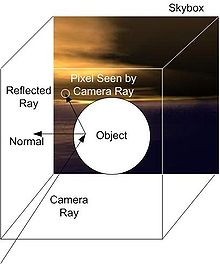
\includegraphics{Cube_mapped_reflection_example}
  \caption{An example of environment mapping. The environment is
    rendered to the sides of the cube and then mapped onto the sphere.
    The mapping is performed by using the calculated reflection vector
    as texture coordinates.}
%TODO image curtesy of http://en.wikipedia.org/wiki/Reflection_mapping
  \label{fig:cubemap}
\end{figure}

An alternative to rasterization is presented by \textit{ray casting}
or \textit{ray tracing}. In ray tracing, each individual pixel is
shaded by tracing one or more \textit{primary rays} ``cast'' from the
camera into the world and observing which primitive they
intersect. Reflection and refraction are easily created by spawning a
new ray at the intersection point and then tracing it. In contrast to
rasterization this provides a much more correct result, easily allows
for multiple \textit{reflection rays} and as we shall see in section
TODO at a much better lower cost increase pr. frame. Shadows are also
easily created using ray tracing. Hard edged shadows can be created by
tracing a \textit{shadow ray} from an intersection point towards a
lightsource. If the shadow ray intersects another part of the world
before it reaches the lightsource, then the intersection point must be
placed in shadow and does not receive any illumination from the
lightsource. Using advanced lighting algorithms such as \textit{photon
  mapping}, which incorporates ray tracing for light transportation,
lighting from reflective surfaces, color bleeding and even correct
caustics can be simulated.

\begin{figure}
  \centering
  
  \subfloat[A cubemapped reflecting dragon.]{
    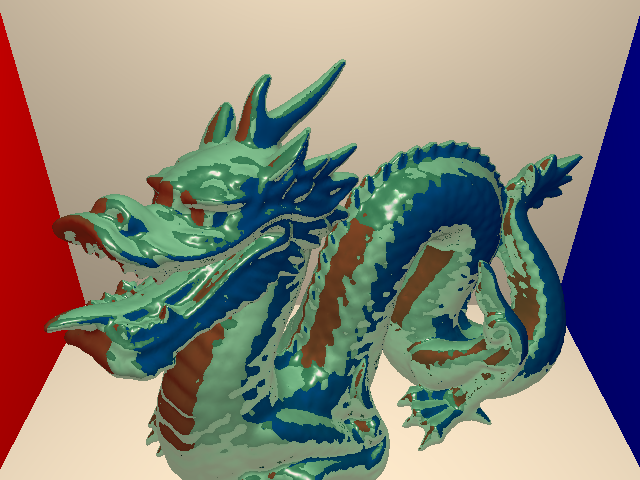
\includegraphics[width=6cm]{cubemappedDragon}
    \label{fig:cubeDragon}
  }

  \subfloat[A ray traced reflecting dragon. Notice the self reflecting
  on the back and inside the mouth.]{
    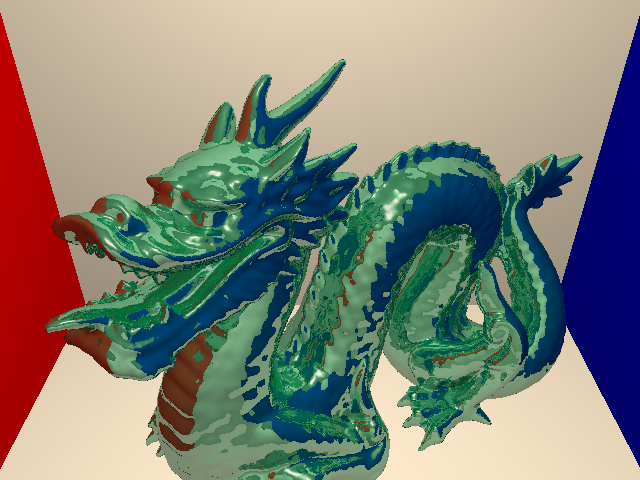
\includegraphics[width=6cm]{semiReflectingDragon}
    \label{fig:rayReflectingDragon}
  }
  \label{fig:reflectingDragons}
\end{figure}

%% \begin{figure}
%%   \centering

%%   \subfloat[A Whiskey Glass rendered by Zhou et al.\citebook{1409079}
%%     using ray tracing and photon mapping. The scene includes shadow,
%%     reflection and refraction rays, aswell as caustics from light rays
%%     passing through the glass and whiskey, as can be seen on table.]{
%%     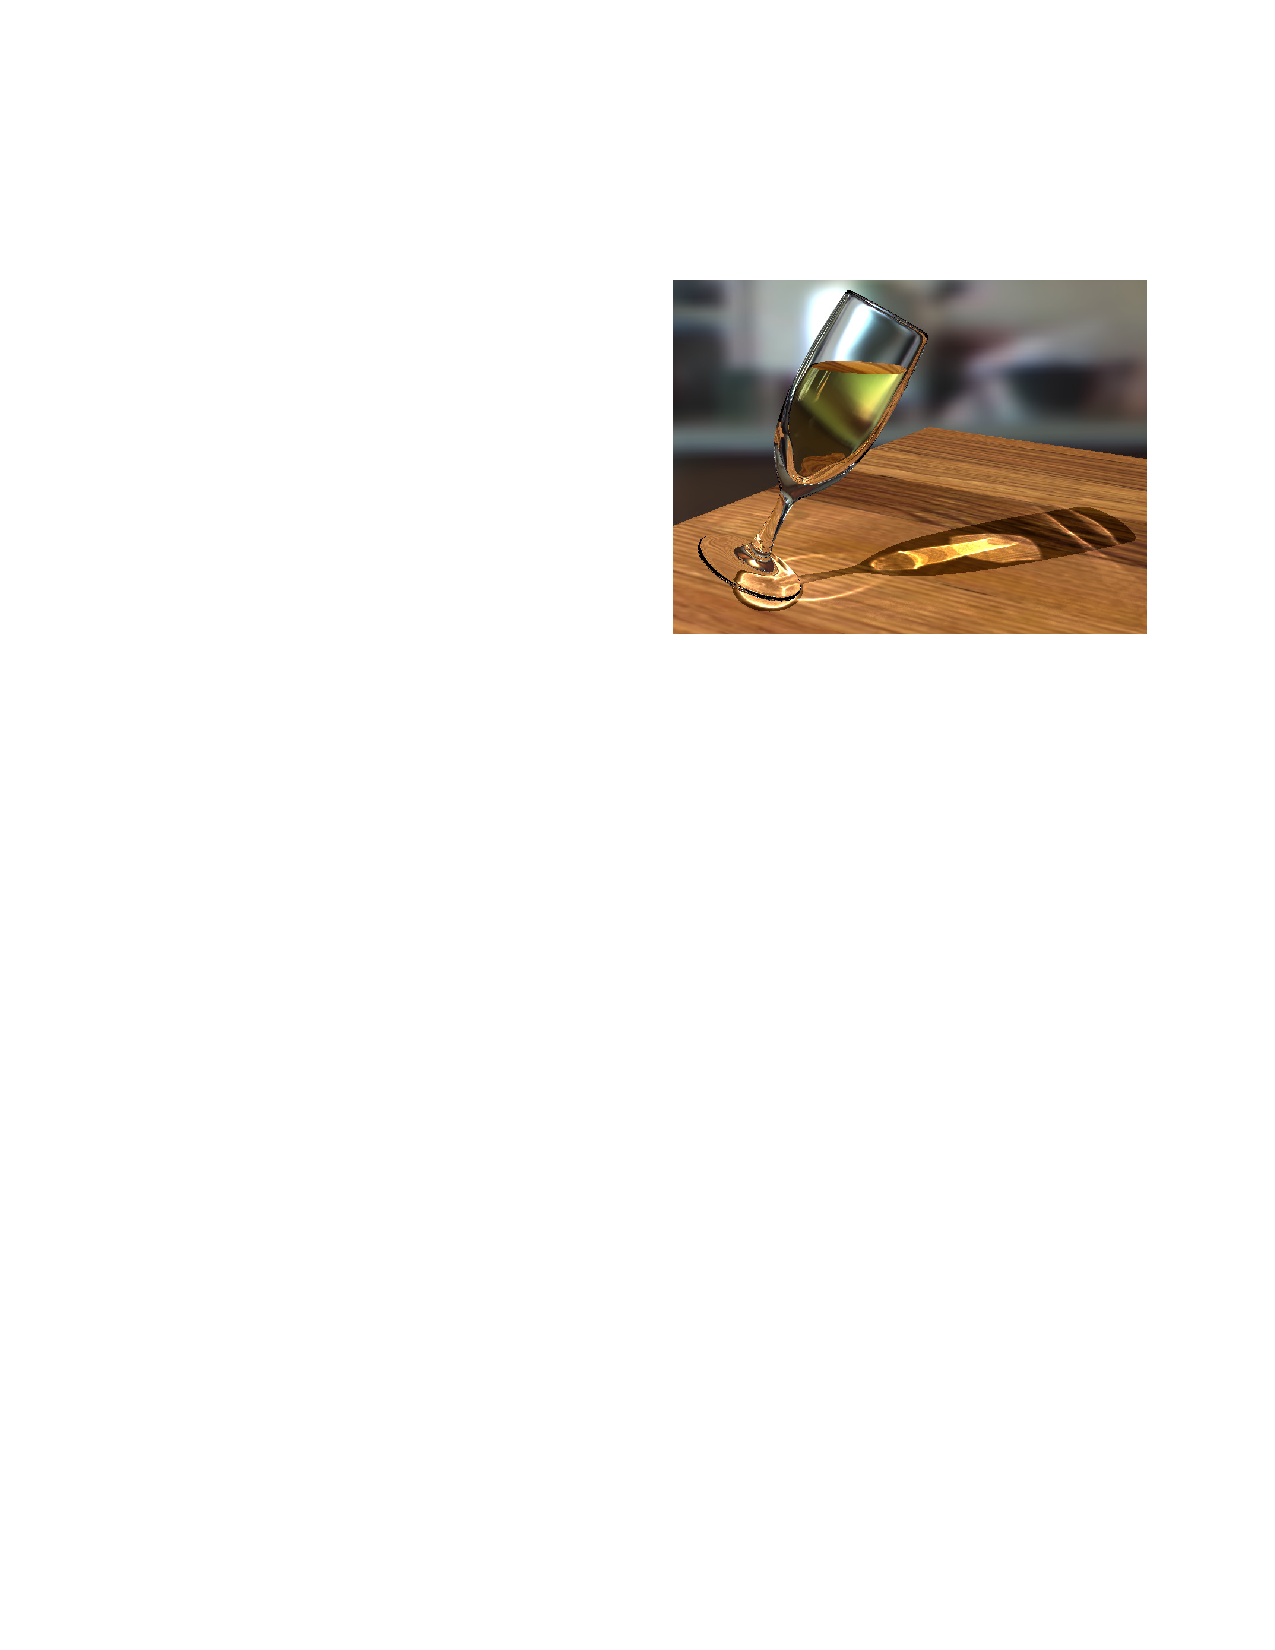
\includegraphics[height=5cm]{WhiskeyGlass}
%%     \label{fig:PhotonGlass}
%%   }

%%   \subfloat[A glass of whiskey from a cutscene in StarCraft 2,
%%     rendered with OpenGL. A reasonable approximation to refraction can
%%     be seen on the glass sides, but the missing caustics leave the
%%     table looking flat. This is especially noticeable when the glass is
%%     moved.]{ 
%%     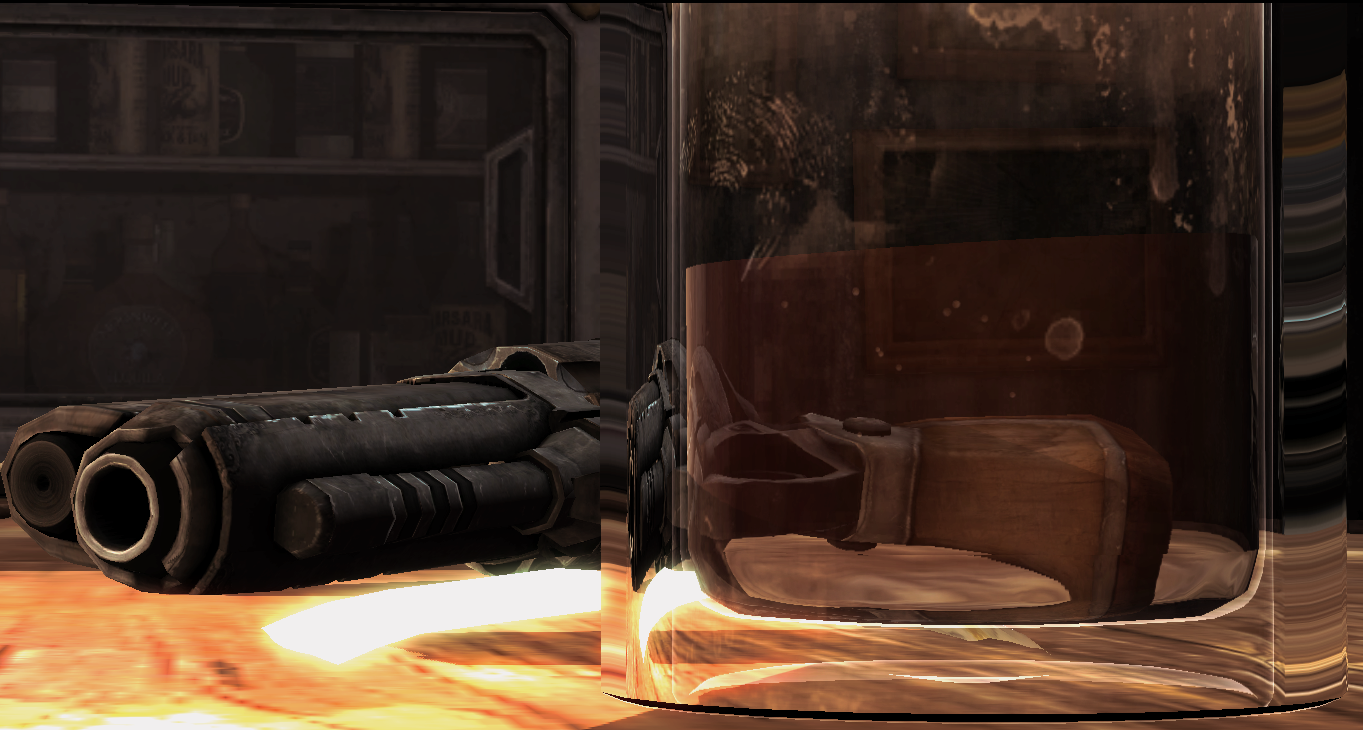
\includegraphics[height=5cm]{StarcraftGlass}
%%     \label{fig:StarCraftGlass}
%%   }
%%   \caption{Examples of a whiskey glass rendered with OpenGL and Photon
%%   Mapping.}
%%   \label{fig:caustics}
%% \end{figure}


Nevertheless, the photorealistic images rendered by ray tracers does
come at a high computational cost, which is why ray tracing is mostly
used for \textit{offline rendering}, for example for special effects in
movies or high quality images.

% Due to increase on computing power, we're getting closer and closer
% to seeing real-time ray tracing and it's lighting in
% applications. Bla bla rewrite!

% The evergrowing interest in photorealistic rendering and the
% complexity of the scenes rendered.

But, due to the everincreasing computational power and continued
research into \textit{global illumination acceleration techniques},
the physically correct image quality obtainable though ray tracing is
becoming more and more alluring to designers of real-time graphical
applications, especially if correct reflection or refraction is
needed.

% Why global illumination vs local illumination used in most
% rasterizers. Ray tracing can produce more correct images, and it
% scales $O(N log M)$, whereas rasterizers scale O(NM) or O(N+M).

TODO time complexity?

% Why use the GPU? Offloading. The CPU can do a lot of other things
% while the GPU crunch away at those KD trees. Om nom nom nom
% nom.... Games already make heavy use of the CPU for game logics,
% networking and AI, they need to offload graphics to the another
% processing unit.

In this thesis I will be combining the rendering quality of ray
tracing with the computational power of modern
\textit{GPGPU}'s\footnote{General Purpose Graphics Processing
  Units.}. This requires that the algorithms presented exploit the
massively dataparallel nature of the graphics card, requiring
thousands of threads for each GPGPU program. This subject will be
discussed in \refchapter{chp:GPGPU}

There are several good reasons for using GPGPU's for ray tracing. Each
ray can be traced independently and in parallel with all the other
rays. Even at a resolution of 512x512, 262144 primary rays are
generated, resulting in more than enough threads to potentionally
utilize all of the GPGPU's multiprocessors. In the case of computer
games, the CPU is already heavily occupied with \textit{game logic},
\textit{networking}, \textit{AI}\footnote{Artificial Intelligence},
and more to also handle rendering, in which case offloading to an
otherwise idle GPGPU only makes sense. Recent advances in GPGPU ray
tracing have also shown performance comparable to CPU
implementations\citebook{1230129}\citebook{popov:07:GPURT}, meaning
the choice of architecture can now be based purely on where most
performance will be available.

Recent advances in acceleration structure creation have allowed them
to be created equally fast on the CPU and
GPGPU\citebook{1409079}. Therefore, as with ray tracing, this thesis
will focus on a GPGPU implementation, to reduce the workload of the
CPU. Keeping the entire workload on the graphics card has the added
benefit of minimizing datatransfers over the bus.

% In this thesis I present an exhaustive ray tracer and compared it to
% a basic non optimized ray tracer traversing a KD-tree, to emphasize
% the importance of datastructures, even on the GPU.

% importance of efficient datastructures, several datastructures have
% been used for ray tracing (BVH, kd-trees, octrees, bla bla...) Some
% are good for bla, others blank

% Reference the 'good' kd tree double speed up and how it doesn't say
% anything about the extra time spend on these good tree.

\quotebook{With todays's fast ray tracers, the difference between a
  ``good'' and a naïvely built kd-tree is often a factor of 2 or
  more.}{wald:06:NlogN}

% can be done by parallising the evaluation of the approximate cost of
% each node

% \textit{Surface Area Heuristic}, $SAH$, 

% and creation of nodes at lower tree levels

% Still not easily paralisable, requires lots of reduction kernels,
% which do not utilize the GPU fully. Also individual node splitting
% costs can leave 31 threads in a warp waiting for the last one to
% finish.

\section{Goals}

In this thesis the goal is not to produce images of photorealistic
quality, or create an interactive ray tracer for dynamic
scenes \footnote{This goal in itself can trivially be achieved by
  reducing the complexity of the scene or lowering the resolution.}
Instead this thesis will explorer ray tracing acceleration structures,
specifically the \textit{kd-tree}\footnote{A \textit{binary space
    partition} tree that is recursively subdivided by splitting the
  geometry.}, and it's impact on ray tracing efficiency for dynamic
scenes.

TODO Quick explanation of what a kd-tree is, with figure? Including
bounding box. Probably move this up into the actual intro.

TODO Ray tracing of dynamic scenes ... something about why it's interesting
and that we have to continuously keep the data structure updated.

There are 3 ways to optimize ray tracing with respect to dynamic
scenes. Either optimize the ray tracer, the time it takes to build the
datastructure or optimize the quality of the data structure. During
this thesis I will investigate different aspects of kd-tree
construction, how optimizations to the tree structure affects ray
tracing performance and if the time spend on those optimizations is
returned when ray tracing.

During this I will look at the usefulness of hierachical traversal
on the GPU, given that a binary data structure is not easy for the
GPU to handle and breaks thread coalescence, which is important for
fast memory access. An exhaustive ray tracer, that performs
intersection with all triangles for all rays, will be used to
motivate the use of a hierachical datatstructure, even on the GPU.

The kd-tree used for accelerating ray tracing will be based on the
implementation described by Zhou etal.\citebook{1409079}.
Improvements to the quality of the tree include which algorithm to use
when determining where to divide the scene and \textit{empty space
  splitting}, which facilitates an early out option for the ray
tracer. 

The thesis will also look at alternate ways of assigning triangles to
nodes on each side of the splitting planes. The most common technique
is \textit{triangle splitting}. I propose and investigate 2 different
approches, in which the triangle is not split into new triangles, but
instead merely assigned to both nodes upon overlapping, which should
result in less triangles being created due to splits and thus smaller
kd-trees.

To compare time spend ray tracing with time spend building the
datastructure, I will need to create an optimized
raytracer. Optimizing the ray tracer for this comparison is important,
since the optimized implementation is up to 80\% faster than the basic
implementation, with no added cost to the kd-tree creation.

Optimizations to the ray tracer will be inspired by the work done in
\citebook{1230129}, but also include investigation of optimal
ray/triangle intersection algorithms, an improvement inspired by
empty space splitting during kd-tree creation and simply structuring
the rays in a manner that favors SIMT execution.


% Result evaluation

Ray tracing optimizations will simply be evaluated based on time saved
during ray tracing. Optimizations will be based on improving the
worst case scenarios, ie long rays shooting towards the center of
the scene.

Strategies that optimize the KD-tree will be evaluated based on the
time added to the kd-tree creation phase, and the time saved in the
ray tracing phase.

\section{Overview}

The thesis is structured as follows:

% Previous work

The next section details previous work in the area of ray tracing and
kd-tree construction. This includes a brief history of when ray
tracing was introduced, aswell as key points in time for different
acceleration structures. The last part of this section will focus on
kd-trees and ray tracing on graphics hardware. Changes in this thesis
compared to previous work in the area are also outlined in this
section.

% Understanding the GPGPU

A chapter will then introduce the GPGPU architecture. Here I will
describe \textit{CUDA}'s\footnote{NVIDIA's Compute Unified Device
  Architecture.} thread and memory model. I will then go on to
describe a new primitive as proposed by Sengupta et
al.\citebook{Sengupta:2007}, which will be helpful for performing
scattering and compaction on wide SIMT architectures. Finally this
section will focus on optimization techniques specific to CUDA, which
will be applied incrementally in a case study of a \textit{reduction}
example.

% kd-trees

\refchapter{chp:kdTrees} is then devoted to discussing kd-trees. The
first part of this section deals with the general kd-tree construction
algorith. Here I will present several algorithms for choosing the
splitting plane and discuss 3 different algorithms for associating
triangles with child nodes. The second part of the section deals with
the actual implementation of kd-trees on a SIMT architecture.

% raytracing

Having introduced kd-trees, the next chapter will deal with the
algorithms for traversing such trees and ray tracing the scene. Here
several optimizations to a basic raytracer will be discussed and
incrementally added to the ray tracer. First though, an exhaustive ray
tracer is presented and will be used in the Results chapter to
motivate the use of hierarchical data structures on the GPGPU. This
section also includes a discussion of 2 triangle intersection
algorithms with respect to performance on the GPGPU. The section ends
with a brief discussion of how colors and reflection/refraction
are calculated.

% Results

% Conclusion

% Future work
